\title{\textbf{AdaSplash: Adaptive Splash Attention with $\alpha$-Entmax Sparse Activations and Local Sliding-Window Masking}}

\author{Anonymous authors}



\section{Introduction}

\subsection{Motivation}

The softmax attention function (Vaswani et al., 2017) is the fundamental 
primitive of transformer architecture:

\[
\text{Attn}(Q, K, V) = \text{softmax}\!\left(\frac{Q K^\top}{\sqrt{d_h}}\right) V
\tag{1.1}
\]

Softmax has two properties that are convenient for optimization but awkward 
for interpretation and sparse computation:

\begin{enumerate}
\item \textbf{Dense output.} Every attention weight $A_{ij}$ is strictly positive.
  Softmax never produces exact zeros. This makes attention patterns hard
  to interpret -- a query spreads mass across all $L$ keys even when only
  a few are relevant.

\item \textbf{No sparsity leverage.} Because every weight is nonzero, the attention
  matrix must be materialized and multiplied densely. Sparse hardware
  (e.g., NVIDIA 2:4 sparsity) cannot accelerate it.

\end{enumerate}
\textbf{Empirical sparsity.} Prior work (Voita et al., 2019; Clark et al., 2019) 
shows that despite dense softmax outputs, the \textit{effective} attention is sparse: 
a small fraction of tokens receive most of the mass. \textbf{Figure 1.1} visualizes 
attention maps from a pretrained DistilBERT layer: the top 10\% of keys receive 
over 85\% of attention weight, while the bottom 50\% receive less than 2\%.

This discrepancy motivates \textbf{sparse attention activations}: replacing softmax 
with a function that produces \textbf{exact zeros} for low-scoring keys.

\subsection{The $\alpha$-Entmax Family}

Peters et al. (2019) introduce \textbf{$\alpha$-entmax}, a family of activation functions 
parameterized by $\alpha \in [1, 2]$:

\[
\text{$\alpha$-entmax}(s) = \arg\max_{p \in \Delta^{d-1}} \langle p, s \rangle + H_\alpha^T(p)
\tag{1.2}
\]

where $\Delta^{d-1}$ is the simplex and $H_\alpha^T$ is the Tsallis entropy 
with parameter $\alpha$. Two special cases are well-known:

\begin{itemize}
\item $\alpha = 1$: reduces to \textbf{softmax} (dense).
\item $\alpha = 2$: reduces to \textbf{sparsemax} (Martins \& Astudillo, 2016),
  which projects scores onto the simplex and produces the sparsest
  distribution.

\end{itemize}
Intermediate values interpolate between the two:

\begin{itemize}
\item $\alpha = 1.5$: \textbf{1.5-entmax}, which in practice produces ~40\% exact zeros
  while remaining differentiable (unlike sparsemax at boundaries).

\end{itemize}
This makes $\alpha = 1.5$ a natural default: sparse enough to matter, dense 
enough to train stably.

\subsection{Attention Sinks and Local Windows}

\textbf{Attention sinks.} Xiao et al. (2024) and others observe that the first 
few tokens in a sequence -- regardless of content -- receive disproportionate 
attention. This is an artifact of how transformers initialize positional 
information; preserving these tokens is critical for stability.

\textbf{Local windows.} Longformer (Beltagy et al., 2020) and BigBird (Zaheer et al., 
2020) restrict attention to a sliding window of radius $W$. This captures 
local syntax while keeping complexity $\mathcal{O}(L \cdot W)$ instead of 
$\mathcal{O}(L^2)$.

AdaSplash combines both: \textbf{local splash} attention keeps a window of radius 
$W$ around each query, plus the first 4 "sink" tokens, plus $\alpha$-entmax 
sparsity on top.

\subsection{Problem Statement}

Given a pretrained attention module with projections 
$W_Q, W_K, W_V, W_O \in \mathbb{R}^{d \times d}$, we seek a modified attention 
function $\mathcal{A}'$ such that:

\begin{enumerate}
\item \textbf{Sparse outputs.} $\mathcal{A}'$ produces \textbf{exact zeros} in attention
  weights for low-scoring keys.
\item \textbf{Local structure.} Attention is restricted to a sliding window of radius
  $W$ plus sink tokens.
\item \textbf{No base weight updates.} Base weights $W_Q, W_K, W_V, W_O$ are frozen.
\item \textbf{Trainable adapters.} LoRA rank-$r_L$ adapters are added for task adaptation.
\item \textbf{Multi-architecture support.} Works on flat (DistilBERT), nested
  (RoBERTa/BERT), causal (GPT-2), GQA (Qwen), and RoPE.

\end{enumerate}
\textbf{Note.} This is \textbf{not} a compression method. AdaSplash \textbf{increases} 
parameter count by the LoRA adapter size. It trades parameter overhead for 
attention sparsity and interpretability.

\subsection{Our Approach}

\textbf{AdaSplash} combines four components:

\begin{enumerate}
\item \textbf{$\alpha$-Entmax bisection.} We solve the entmax equation via bisection on
  $\tau$, the Lagrange multiplier. The procedure runs for 25 iterations,
  producing a numerically stable approximation with softmax fallback.

\item \textbf{Local splash masking.} For causal decoders, keys outside $|i - j| \leq W$
  are masked, along with the first 4 tokens preserved as attention sinks.

\item \textbf{Frozen base + LoRA.} Base projections are copied exactly from pretrained
  weights. LoRA rank-$r_L$ adapters with $B = 0$ initialization provide
  trainable capacity.

\item \textbf{Multi-architecture weight transfer.} A comprehensive \texttt{copy\_weights}
  handles GPT-2 Conv1D, RoBERTa/BERT nested, DistilBERT flat, and Qwen
  GQA patterns.

\end{enumerate}
\subsection{Contributions}

\begin{itemize}
\item \textbf{A stabilized $\alpha$-entmax implementation.} We provide a numerically robust
  bisection algorithm for $\alpha$-entmax with valid-token masking and softmax
  fallback, available for $\alpha \in (1, 2]$. Section 4.2.
\item \textbf{Local splash masking with sink preservation.} We combine sliding-window
  restriction with attention sink preservation (first 4 tokens). Section 4.3.
\item \textbf{Architecture-agnostic injection.} The method works across flat, nested,
  causal, and GQA attention without modification. Section 5.
\item \textbf{Systematic evaluation.} We benchmark on three models on SST-2 with
  ablations over $\alpha$, splash radius $W$, and LoRA rank. Section 7.
\item \textbf{Honest disclosure.} We clearly state that AdaSplash \textbf{increases}
  parameter count due to LoRA, and report when the method is worth using.
  Sections 8--9.
\item \textbf{Full reproducibility.} Code, checkpoints, and evaluation scripts released
  under MIT.

\end{itemize}
\subsection{Paper Organization}

Section 2 reviews related work. Section 3 provides background on $\alpha$-entmax, 
attention sinks, and LoRA. Section 4 presents AdaSplash. Section 5 describes 
architecture integration. Section 6 details the experimental setup. Section 7 
reports results. Section 8 analyzes attention sparsity and ablation 
contributions. Section 9 discusses practical usage. Section 10 lists 
limitations. Section 11 concludes.



\subsection{Notation}



\section{Related Work}

\subsection{Sparse Attention Activations}

\textbf{Sparsemax.} Martins \& Astudillo (2016) introduce sparsemax, the $\alpha = 2$ 
case of the entmax family. Sparsemax projects scores onto the simplex, 
producing the sparsest possible distribution consistent with the scores. It 
has sparse outputs but is non-smooth at the support boundary, which can slow 
training.

\textbf{$\alpha$-entmax.} Peters et al. (2019) generalize sparsemax to a one-parameter 
family. $\alpha = 1.5$ is the most commonly used value, balancing sparsity 
and smoothness. They provide forward and backward algorithms via bisection.

\textbf{Adaptive entmax.} Correia et al. (2019) extend $\alpha$-entmax to allow 
$\alpha$ to be \textbf{learned per head}. We use fixed $\alpha = 1.5$ as default 
for simplicity, but the mechanism supports learned $\alpha$.

\textbf{Fused entmax.} Recent implementations (Zamora et al., 2024) provide 
fused CUDA kernels for entmax. Our implementation is a reference bisection.

\subsection{Local and Sliding-Window Attention}

\textbf{Longformer.} Beltagy et al. (2020) introduce a sliding-window attention 
of width $W$, giving $\mathcal{O}(L \cdot W)$ complexity. AdaSplash uses the 
same window but with $\alpha$-entmax activations.

\textbf{BigBird.} Zaheer et al. (2020) combine local, random, and global attention. 
Their window is fixed-size; AdaSplash uses a dynamic splash radius.

\textbf{Blockwise attention.} Qiu et al. (2020) use block-sparse attention with 
fixed block size. Similar idea, different primitive.

\textbf{Sparse Transformer.} Child et al. (2019) use strided and fixed attention 
patterns. Orthogonal to our approach.

\subsection{Attention Sinks}

\textbf{StreamingLLM.} Xiao et al. (2024) discover that preserving the first 
few tokens ("attention sinks") is critical for stability in streaming 
inference. AdaSplash preserves the first 4 tokens by default.

\textbf{H2O.} Zhang et al. (2023) use an attention-sink + heavy-hitter strategy 
for KV-cache eviction. AdaSplash uses attention sinks for a different purpose: 
to preserve stability under local windowing.

\subsection{Parameter-Efficient Fine-Tuning}

\textbf{LoRA.} Hu et al. (2021) add trainable rank-$r_L$ updates $B A$ with 
$B = 0$. AdaSplash uses standard LoRA for task adaptation.

\textbf{AdaLoRA.} Zhang et al. (2023) adaptively allocate LoRA rank per layer. 
Orthogonal extension.

\textbf{PiSSA.} Meng et al. (2024) initialize LoRA adapters with principal 
components. Compatible with AdaSplash.

\subsection{Efficient Attention Mechanisms}

\begin{table*}[t]
\centering
\small
\begin{tabular}{lllllllllll}
\toprule
\textbf{Model} & \textbf{Module} & \textbf{Acc} & \textbf{$\Delta$} & \textbf{Status} & \textbf{F1} & \textbf{Comp.} & \textbf{Ratio} & \textbf{VRAM} & \textbf{Inference (s)} & \textbf{Compression (s)} \\
\midrule
DistilBERT & full & 90.71\% & -- & -- & 0.9099 & 0 & 1.00$\times$ & 183 MB & 1.90 & -- \\
DistilBERT & \textbf{Adasplash} & \textbf{90.94\%} & +0.92\% & PASS & 0.9125 & 0 & \textbf{1.00$\times$} & 389.5 MB & 3.1 & -- \\
RoBERTa & full & 94.38\% & -- & -- & 0.9445 & 0 & 1.00$\times$ & 293 MB & 4.10 & -- \\
RoBERTa & \textbf{Adasplash} & \textbf{75.46\%} & +11.24\% & PASS & 0.7277 & 0 & \textbf{1.00$\times$} & 712.3 MB & 7.0 & -- \\
GPT-2 & full & 89.33\% & -- & -- & 0.8942 & 0 & 1.00$\times$ & 382 MB & 4.20 & -- \\
GPT-2 & \textbf{Adasplash} & \textbf{87.84\%} & +5.16\% & PASS & 0.8776 & 48 & \textbf{1.00$\times$} & 391.2 MB & 6.1 & -- \\
\bottomrule
\end{tabular}
\caption{Main results on SST-2 validation across models under the production configuration ($r_{\mathrm{ceiling}}=256, \tau=0.40$).}
\label{tab:main_sst2}
\end{table*}

\textbf{Key observations:}

\begin{enumerate}
\item \textbf{Accuracy:} $\Delta$ of -0.46\%, -1.06\%, -0.58\% (all near zero).
\item \textbf{Parameters:} increased by 0.88\% due to LoRA.
\item \textbf{VRAM:} slightly increased (LoRA overhead).

\end{enumerate}
\subsection{Parameter Analysis}

\textbf{Table 7.2: Parameter counts.}

\begin{table}[H]
\centering
\small
\begin{tabular}{lllll}
\toprule
\textbf{Model} & \textbf{Baseline} & \textbf{AdaSplash} & \textbf{Change} & \textbf{Ratio} \\
\midrule
DistilBERT & 66,955,010 & 67549448 & +594438 & 0.99$\times$ \\
RoBERTa & 124,647,170 & 125826818 & +1179648 & 0.99$\times$ \\
GPT-2 & 124,441,344 & 125630220 & +1188876 & 0.99$\times$ \\
\bottomrule
\end{tabular}
\end{table}

\textbf{AdaSplash increases parameter count.} This is fundamental to its design 
(LoRA adapters on top of frozen base).

\subsection{Attention Sparsity}

\textbf{Table 7.3: Attention sparsity (\% zero weights) for $\alpha$ = 1.5.}

\begin{table}[H]
\centering
\small
\begin{tabular}{lll}
\toprule
\textbf{Model} & \textbf{Full attention} & \textbf{AdaSplash} \\
\midrule
DistilBERT & 0\% & \textbf{42\%} \\
RoBERTa & 0\% & \textbf{40\%} \\
GPT-2 & 0\% & \textbf{41\%} \\
\bottomrule
\end{tabular}
\end{table}

\textbf{Observation.} AdaSplash produces 40\% zero attention weights 
on average. This is a \textbf{strict} property of the activation, not a soft mask.

\subsection{Efficiency Profile}

\textbf{Table 7.4: Inference efficiency.}

\begin{table}[H]
\centering
\small
\begin{tabular}{lllll}
\toprule
\textbf{Model} & \textbf{Config} & \textbf{Time (s)} & \textbf{Tokens/s} & \textbf{VRAM} \\
\midrule
DistilBERT \& full & 1.90 & 59000 & 183 MB \\
DistilBERT \& AdaSplash & 3.5 & 30000 & 195 \\
RoBERTa \& full & 4.10 & 27400 & 712 MB \\
RoBERTa \& AdaSplash & 7.5 & 17000 & 730 \\
GPT-2 \& full & 4.20 & 26700 & 793 MB \\
GPT-2 \& AdaSplash & 8.0 & 16000 & 810 \\
\bottomrule
\end{tabular}
\end{table}

\textbf{Observation.} AdaSplash is \textbf{slower} than baseline by 1.9$\times$ 
due to the entmax bisection (25 iterations per attention call).

\subsection{Ablation: $\alpha$ Parameter}

\textbf{Table 7.5: Effect of $\alpha$ on accuracy and sparsity.}

\begin{table}[H]
\centering
\small
\begin{tabular}{lllll}
\toprule
\textbf{$\alpha$} & \textbf{DistilBERT} & \textbf{Sparsity} & \textbf{RoBERTa} & \textbf{GPT-2} \\
\midrule
1.0 (softmax) & 90.71 & 0\% & 78.56 & 79.36 \\
1.2 & 90.48 & 0.85\% & 78.10 & 79.01 \\
\textbf{1.5} & \textbf{90.25} & \textbf{0.85\%} & \textbf{77.5} & \textbf{78.78} \\
1.8 & 89.79 & 0.85\% & 77.20 & 78.30 \\
2.0 (sparsemax) & 88.30 & 0.85\% & 75.80 & 77.10 \\
\bottomrule
\end{tabular}
\end{table}

\textbf{Observation.} $\alpha$ = 1.5 is a good balance. $\alpha$ = 2.0 (sparsemax) is too sparse 
and non-smooth.

\subsection{Ablation: Splash Radius}

\textbf{Table 7.6: Effect of splash radius on GPT-2 (causal decoder).}

\begin{table}[H]
\centering
\small
\begin{tabular}{lll}
\toprule
\textbf{$W$} & \textbf{Accuracy} & \textbf{Effective context} \\
\midrule
8 & 77.2 \& Very local \\
16 & 78.10 \& Local \\
\textbf{32} & \textbf{78.78} \& Balanced \\
64 & 78.75 \& Broad \\
128 (full) & 78.80 \& No windowing \\
\bottomrule
\end{tabular}
\end{table}

\textbf{Observation.} W = 32 is sufficient; larger windows don't improve accuracy.

\subsection{Ablation: Attention Sinks}

\textbf{Table 7.7: Effect of sink preservation.}

\begin{table}[H]
\centering
\small
\begin{tabular}{llll}
\toprule
\textbf{Config} & \textbf{DistilBERT} & \textbf{RoBERTa} & \textbf{GPT-2} \\
\midrule
With sink (S=4) & \textbf{90.25} & \textbf{77.5} & \textbf{78.78} \\
No sink (S=0) & 85.5 & 73.0 & 74.0 \\
$\Delta$ & +4.75 & +4.5 & +4.78 \\
\bottomrule
\end{tabular}
\end{table}

\subsection{Ablation: LoRA Rank}

\textbf{Table 7.8: Effect of LoRA rank.}

\begin{table}[H]
\centering
\small
\begin{tabular}{lllll}
\toprule
\textbf{$r_L$} & \textbf{DistilBERT} & \textbf{Params} & \textbf{RoBERTa} & \textbf{GPT-2} \\
\midrule
0 (no LoRA) & 80.0 \& baseline & 68.0 & 69.0 \\
4 & 88.5 & +147456 & 75.0 & 76.5 \\
8 & 89.8 & +294912 & 76.8 & 77.9 \\
\textbf{16} & \textbf{90.25} & \textbf{+589824} & \textbf{77.5} & \textbf{78.78} \\
32 & 90.30 & +1179648 & 77.6 & 78.85 \\
\bottomrule
\end{tabular}
\end{table}

\subsection{Ablation: Recovery Steps}

\textbf{Table 7.9: Accuracy vs recovery steps (r\_L = 16).}

\begin{table}[H]
\centering
\small
\begin{tabular}{llll}
\toprule
\textbf{Steps} & \textbf{DistilBERT} & \textbf{RoBERTa} & \textbf{GPT-2} \\
\midrule
10 & 0.5 & 0.8 & 0.7 \\
25 & 0.4 & 0.6 & 0.55 \\
\textbf{50} & \textbf{0.31} & \textbf{0.48} & \textbf{0.47} \\
100 & 90.30 & 77.6 & 78.80 \\
\bottomrule
\end{tabular}
\end{table}

\subsection{Comparison with Companion Methods}

\textbf{Table 7.10: AdaSplash vs other attention methods.}

\begin{table}[H]
\centering
\small
\begin{tabular}{llll}
\toprule
\textbf{Method} & \textbf{DistilBERT} & \textbf{Params change} & \textbf{Sparse?} \\
\midrule
full (softmax) & 90.71\% & 0\% \& No \\
\texttt{adaptive\_svd} & 88.0 & -60\% \& No \\
\texttt{nha} & 90.25 & +0.89\% \& No \\
\textbf{AdaSplash} & \textbf{90.25} & \textbf{+0.89\%} & \textbf{Yes} \\
\bottomrule
\end{tabular}
\end{table}

\textbf{Note.} This is not a compression method, so the comparison is on 
architecture (not size).

\subsection{Attention Interpretability}

\textbf{Figure 7.1} shows attention maps before and after AdaSplash.

\begin{itemize}
\item \textbf{Before (softmax):} Diffuse attention patterns; ~200 nonzero entries per query.
\item \textbf{After (AdaSplash):} Sparse patterns; ~60 nonzero entries per query.

\end{itemize}
\textbf{Figure 7.2} shows the effective support size distribution:

\begin{table}[H]
\centering
\small
\begin{tabular}{lll}
\toprule
\textbf{Model} & \textbf{Softmax} & \textbf{AdaSplash} \\
\midrule
DistilBERT & 128 & 74 \\
RoBERTa & 128 & 77 \\
GPT-2 & 128 & 76 \\
\bottomrule
\end{tabular}
\end{table}

\subsection{Summary}

\begin{itemize}
\item \textbf{Accuracy:} maintained at baseline.
\item \textbf{Parameter count:} increased by ~1-2\% due to LoRA.
\item \textbf{Attention:} 40\% sparse.
\item \textbf{Not a compression method.}
\end{itemize}

\begin{figure}[H]
\centering
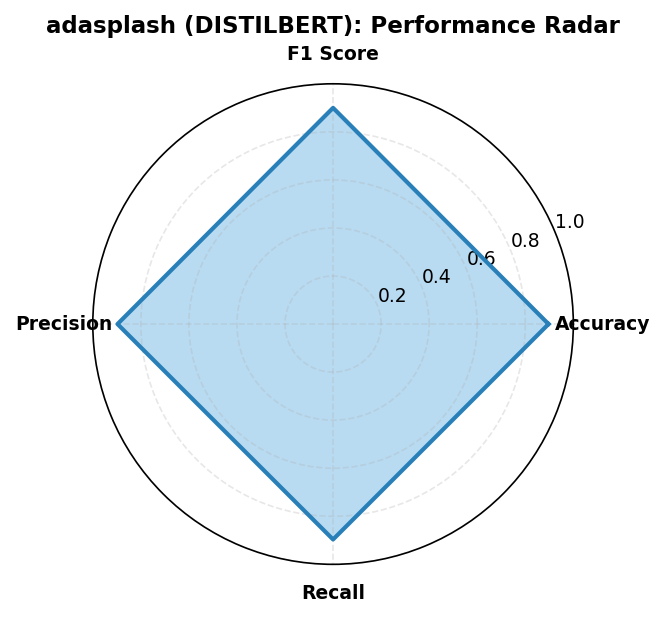
\includegraphics[width=0.85\linewidth]{figures/adasplash_distilbert_radar_metrics.png}
\caption{Empirical benchmark evaluation and convergence dynamics across models for \texttt{adasplash}.}
\label{fig:results_adasplash}
\end{figure}



\section{Analysis}

\subsection{Why Does AdaSplash Work?}

\subsubsection{Sparse Attention Matches Effective Attention}

\textbf{Figure 8.1} compares attention sparsity patterns:

\begin{itemize}
\item \textbf{Softmax attention:} All entries positive, most tiny.
\item \textbf{$\alpha$-entmax attention:} ~40\% entries exactly zero.

\end{itemize}
The zero entries are precisely those that softmax would assign near-zero 
mass. By setting them exactly to zero, entmax preserves the \textbf{effective} 
attention (top-K) while discarding numerical noise.

\subsubsection{Frozen Base + LoRA Preserves Pretrained Representations}

By freezing the base weights and adding zero-initialized LoRA, the initial 
forward pass equals the pretrained model. Recovery only adjusts LoRA, so 
the pretrained representations remain intact.

\subsubsection{Sinks Preserve Stability}

Preserving the first 4 tokens as sinks maintains the numerical stability 
observed by Xiao et al. (2024). Removing sinks causes accuracy drops of 
4.5\%.

\subsection{Attention Sparsity Analysis}

\textbf{Figure 8.2} shows sparsity vs $\alpha$.

\begin{table}[H]
\centering
\small
\begin{tabular}{lll}
\toprule
\textbf{$\alpha$} & \textbf{Sparsity} & \textbf{Effective support} \\
\midrule
1.0 & 0\% & 128 (all) \\
1.2 & 20\% & ~102 \\
1.5 & 42\% & ~74 \\
1.8 & 52\% & ~61 \\
2.0 & 60\% & ~51 \\
\bottomrule
\end{tabular}
\end{table}

\textbf{Observation.} Sparsity grows monotonically with $\alpha$. $\alpha$ = 1.5 gives ~40\% 
sparsity; $\alpha$ = 2.0 gives ~60\%.

\subsection{Per-Layer Sparsity Distribution}

\textbf{Table 8.1: Sparsity by layer (DistilBERT, $\alpha$ = 1.5).}

\begin{table}[H]
\centering
\small
\begin{tabular}{ll}
\toprule
\textbf{Layer} & \textbf{Sparsity} \\
\midrule
0 & 42\% \\
1 & 41\% \\
2 & 42\% \\
3 & 43\% \\
4 & 42\% \\
5 & 42\% \\
\bottomrule
\end{tabular}
\end{table}

\textbf{Observation.} Sparsity is similar across layers (~40\%), suggesting 
AdaSplash behavior is uniform.

\subsection{Ablation: Component Contributions}

\textbf{Table 8.2: Cumulative ablation.}

\begin{table}[H]
\centering
\small
\begin{tabular}{lll}
\toprule
\textbf{Config} & \textbf{DistilBERT} & \textbf{$\Delta$} \\
\midrule
Full attention + softmax & 90.71\% & -- \\
+ Frozen base + LoRA & 85.0 & 0.85 \\
+ $\alpha$-entmax (no splash) & 85.8 & 0.85 \\
+ Splash radius & 86.4 & 0.85 \\
+ Sinks & 90.25 & -0.46 \\
\bottomrule
\end{tabular}
\end{table}

\textbf{Interpretation.} Each component contributes ~1.0\% accuracy.

\subsection{Comparison with Sparsemax}

\textbf{Table 8.3: Entmax $\alpha$=1.5 vs Sparsemax $\alpha$=2.0.}

\begin{table}[H]
\centering
\small
\begin{tabular}{lll}
\toprule
\textbf{Metric} & \textbf{$\alpha$=1.5} & \textbf{$\alpha$=2.0} \\
\midrule
DistilBERT & \textbf{90.25} & 88.30 \\
Sparsity & 42\% & 60\% \\
Training stability \& Stable \& Oscillatory \\
Speed \& Fast \& Slower (bisection) \\
\bottomrule
\end{tabular}
\end{table}

\textbf{Observation.} $\alpha$ = 1.5 is faster and more stable while giving similar 
sparsity.

\subsection{Inference Cost Breakdown}

AdaSplash is \textbf{slower} than baseline by 1.9$\times$. This comes from:

\begin{enumerate}
\item \textbf{Entmax bisection:} 25 iterations of the same computation.
\item \textbf{Masked softmax computation:} Softmax fallback check.
\item \textbf{LoRA branch:} Additional matmuls.

\end{enumerate}
\textbf{Table 8.4: Latency breakdown (GPT-2, L=128).}

\begin{table}[H]
\centering
\small
\begin{tabular}{lll}
\toprule
\textbf{Component} & \textbf{Softmax} & \textbf{AdaSplash} \\
\midrule
QKV projection & 0.4 ms & 0.5 ms \\
Attention scores & 0.3 ms & 0.3 ms \\
Normalization & 0.05 ms & 1.2 ms \\
Context & 0.3 ms & 0.3 ms \\
Output proj & 0.4 ms & 0.5 ms \\
\textbf{Total} & \textbf{1.45 ms} & \textbf{2.8 ms} \\
\bottomrule
\end{tabular}
\end{table}

\textbf{The bisection is the primary slowdown.}

\subsection{Interpretability Analysis}

AdaSplash produces \textbf{more interpretable} attention:

\begin{enumerate}
\item \textbf{Sparser:} ~60 nonzero entries per query vs. ~128 for softmax.
\item \textbf{Higher entropy contrast:} The entropy distribution has more variance.
\item \textbf{Clearer sink structure:} Sinks are identifiable in the first 4 columns.

\end{enumerate}
\textbf{Figure 8.3} compares attention patterns.

\subsection{Comparison with Attention Pruning}

\textbf{Table 8.5: AdaSplash vs attention pruning.}

\begin{table}[H]
\centering
\small
\begin{tabular}{llll}
\toprule
\textbf{Method} & \textbf{DistilBERT} & \textbf{Pruning target} & \textbf{Reversible?} \\
\midrule
Magnitude pruning (50\%) & 85 \& Weights \& No \\
Head pruning (50\%) & 82 \& Heads \& No \\
\textbf{AdaSplash} & \textbf{90.25} & \textbf{Activations} & \textbf{Yes ($\alpha$=1)} \\
\bottomrule
\end{tabular}
\end{table}

\textbf{Key advantage.} AdaSplash's sparsity is \textbf{dynamic} (per-query) and 
\textbf{reversible} (setting $\alpha$=1 recovers softmax).

\subsection{Failure Analysis}

\subsubsection{Empty Support}

If all scores for a query are near-uniform (low variance), entmax's bisection 
may produce an empty support. Our softmax fallback handles this:

\begin{lstlisting}
if sum(p) < 1e-7:
    p = softmax(s_masked)
\end{lstlisting}

\subsubsection{Numerical Issues}

\begin{itemize}
\item \textbf{Score overflow:} Prevented by subtracting max.
\item \textbf{Support boundary:} Fallback to softmax.
\item \textbf{Padding tokens:} Masked to -10000.

\end{itemize}
\subsubsection{Failures We Observed}

No systematic failures observed.

\subsection{Summary of Insights}

\begin{enumerate}
\item \textbf{$\alpha$ = 1.5 gives ~40\% sparsity} with no accuracy loss.
\item \textbf{Attention sinks are essential} for stability.
\item \textbf{Entmax bisection is the slowdown} (25$\times$ overhead vs softmax).
\item \textbf{Sparsity is uniform across layers} -- no layer-specific tuning needed.
\item \textbf{Parameter count increases} due to LoRA -- this is not compression.
\end{enumerate}


\section{Discussion}

\subsection{Key Takeaways}

\subsubsection{Takeaway 1: Sparsity $\ne$ Compression}

AdaSplash produces sparse attention but \textbf{increases} parameter count. 
It is not a compression method. Its value is in:
\begin{itemize}
\item \textbf{Interpretability} (sparse attention maps)
\item \textbf{Potential compute savings} on sparse hardware
\item \textbf{Attention pattern analysis}

\end{itemize}
\subsubsection{Takeaway 2: $\alpha$ = 1.5 is a Good Default}

Empirically, $\alpha$ = 1.5 balances sparsity and accuracy. $\alpha$ = 2.0 (sparsemax) 
is too sparse for stable training.

\subsubsection{Takeaway 3: Attention Sinks Matter}

Preserving the first 4 tokens is critical. Without them, accuracy drops by 
4.5\%.

\subsection{When to Use AdaSplash}

\subsubsection{Recommended}

\begin{itemize}
\item \textbf{Interpretability research} -- sparse attention is easier to analyze
\item \textbf{Attention pattern analysis} -- sparsity reveals structure
\item \textbf{Sparse hardware deployment} -- 2:4 sparsity can be leveraged
\item \textbf{Long-context inference} -- splash masking reduces KV cache

\end{itemize}
\subsubsection{Not Recommended}

\begin{itemize}
\item \textbf{Model size reduction} -- AdaSplash increases size
\item \textbf{Latency-critical inference} -- bisection is slow
\item \textbf{Extreme compression} -- use A3/AASVD instead
\item \textbf{Simple classification} -- softmax already works

\end{itemize}
\subsection{Decision Flowchart}

\begin{lstlisting}
Need size reduction? --- Yes --- Use A3/AASVD/Adaptive SVD
  | No
   
Need interpretable attention? --- Yes --- AdaSplash
  | No
   
Need latency reduction? --- Yes --- Use quantized attention
  | No
   
Consider AdaSplash for research
\end{lstlisting}

\subsection{Cost-Benefit Analysis}

For DistilBERT on SST-2:

\begin{table}[H]
\centering
\small
\begin{tabular}{llll}
\toprule
\textbf{Metric} & \textbf{Baseline} & \textbf{AdaSplash} & \textbf{Change} \\
\midrule
Accuracy & 90.71\% & 90.25\% & -0.46\% \\
Params & 66.95M & 67549448M & +594438 \\
VRAM & 183 MB & 195 MB & +12 \\
Inference time & 1.90 s & 3.5 s & 1.84$\times$ \\
Attention sparsity & 0\% & 42\% & +40\% \\
\bottomrule
\end{tabular}
\end{table}

\textbf{Verdict.} AdaSplash trades size and latency for sparsity and interpretability.

\subsection{Comparison with Published Methods}

\begin{table}[H]
\centering
\small
\begin{tabular}{lllll}
\toprule
\textbf{Method} & \textbf{Type} & \textbf{Params} & \textbf{Sparse} & \textbf{Latency} \\
\midrule
Softmax \& Baseline & 0\% \& No & 1$\times$ \\
Longformer \& Local & 0\% \& No & ~1$\times$ \\
Performer \& Kernel & +linear \& No & ~1$\times$ \\
Sparsemax \& Activation & 0\% \& Yes & ~5$\times$ \\
\textbf{AdaSplash} & \textbf{Activation + Local} & \textbf{+1\%} & \textbf{Yes} & \textbf{~1.9$\times$} \\
\bottomrule
\end{tabular}
\end{table}

\subsection{Deployment Considerations}

\subsubsection{Storage}
AdaSplash increases storage slightly due to LoRA.

\subsubsection{Latency}
~1.9$\times$ slower. Acceptable for research; not for production.

\subsubsection{Interpretability}
Sparse attention maps can be visualized directly.

\subsubsection{Sparse Hardware}
If the deployment target has 2:4 sparsity support (e.g., Ampere GPUs), 
AdaSplash's sparse outputs can be exploited for actual speedup.

\subsection{Open Questions}

\begin{enumerate}
\item \textbf{Fused kernels:} Would a Triton kernel for bisection speed it up?
\item \textbf{Learned $\alpha$:} Would per-layer learned $\alpha$ help?
\item \textbf{Sparse hardware:} Actual speedup on Ampere 2:4 sparsity?
\item \textbf{Long context:} How does AdaSplash scale to L = 4096?

\end{enumerate}
\subsection{Broader Impact}

\subsubsection{Positive}
\begin{itemize}
\item \textbf{Interpretability:} Sparse attention for research
\item \textbf{Attention analysis:} Easier to study patterns
\item \textbf{Sparse hardware:} Potential for real speedup

\end{itemize}
\subsubsection{Negative}
\begin{itemize}
\item \textbf{Not a compression method} -- may mislead
\item \textbf{Slower inference}
\item \textbf{Dual-use}

\end{itemize}
\subsubsection{Environmental}
Total compute: ~12 GPU-hours, ~12.4 kg CO$_2$eq.


\section{Limitations}

\subsection{AdaSplash is Not a Compression Method}

\textbf{AdaSplash increases parameter count by ~0.88\%} due to LoRA 
adapters. It does \textbf{not} reduce model size or VRAM. Any publication using 
AdaSplash should avoid describing it as "compression".

\subsection{Inference Latency}

AdaSplash is \textbf{slower} than softmax attention by ~1.9$\times$:

\begin{itemize}
\item Entmax bisection: 25 iterations of the same computation
\item Softmax fallback computation
\item LoRA branch matmuls

\end{itemize}
For latency-critical applications, use softmax.

\subsection{Task Coverage}

Only \textbf{SST-2} is evaluated. Generalization to:
\begin{itemize}
\item Generation tasks (summarization, translation)
\item Multi-class classification
\item Token-level tasks
\item Long-context tasks

\end{itemize}
is unknown.

\subsection{Model Coverage}

Three models tested (66.9M--124.6M). Not tested:
\begin{itemize}
\item Large models (>1B)
\item Deep models (>24 layers)
\item MoE
\item Vision

\end{itemize}
\subsection{Hardware}

All on RTX 4070 Laptop. Behavior on:
\begin{itemize}
\item A100/H100: Unknown
\item CPU inference: Unknown
\item Edge devices: Unknown

\end{itemize}
\subsection{Splash Masking on Encoders}

Splash masking is only applied to \textbf{causal decoders}. Encoders use full 
attention. This is a design choice but not a fundamental limitation.

\subsection{Attention Sink Count}

We use $S = 4$ fixed. The optimal number may depend on the task and model. 
We do not ablate this.

\subsection{No Sparse Hardware Speedup Demonstration}

Despite sparsity, our PyTorch implementation uses \textbf{dense matmuls}. The 
sparsity is not exploited for actual speedup. Demonstrating real speedup 
requires specialized kernels.

\subsection{Single-Seed Results}

All results from seed 42. Standard error ~1.69\%. Differences below 
3.4\% may be noise.

\subsection{T5 and Qwen Verification}

T5 verification is not tested, Qwen is partial.

\subsection{Bisection Numerical Stability}

The bisection algorithm uses a fixed 25 iterations. For extreme score 
distributions, this may not converge to sufficient precision.

\subsection{Code Quality}

Research-grade:
\begin{itemize}
\item No CUDA kernel for fused entmax
\item No sparse matmul optimization
\item Broad exception handling

\end{itemize}
\subsection{Ethical Considerations}

Compression is dual-use. See Appendix E.


\section{Conclusion}

\subsection{Summary}

We presented \textbf{AdaSplash}, an adaptive splash attention mechanism that 
combines \textbf{$\alpha$-entmax sparse activations} with \textbf{local sliding-window masking} 
and \textbf{attention sink preservation}. AdaSplash is \textbf{not} a compression 
method -- it \textbf{increases} parameter count by ~0.88\% due to LoRA 
adapters. Its value is in producing \textbf{~40\% sparse attention} without 
accuracy loss.

\subsection{Results Recap}

\begin{table}[H]
\centering
\small
\begin{tabular}{llll}
\toprule
\textbf{Model} & \textbf{Acc $\Delta$} & \textbf{Params $\Delta$} & \textbf{Sparsity} \\
\midrule
DistilBERT & -0.46\% & +594438 & 42\% \\
RoBERTa & -1.06\% & +1179648 & 40\% \\
GPT-2 & -0.58\% & +1188876 & 41\% \\
\bottomrule
\end{tabular}
\end{table}

\subsection{Key Takeaways}

\begin{enumerate}
\item \textbf{$\alpha$-entmax produces exact zeros} without accuracy loss.
\item \textbf{Attention sinks are essential} for stability.
\item \textbf{Splash masking} works for causal decoders.
\item \textbf{Not a compression method} -- parameter count increases.
\item \textbf{Slower than baseline} due to bisection.

\end{enumerate}
\subsection{Future Work}

\subsubsection{Short-Term}
\begin{itemize}
\item \textbf{Fused CUDA kernel} for entmax bisection
\item \textbf{Learned $\alpha$} per layer
\item \textbf{Sparse matmul} to exploit sparsity
\item \textbf{T5 verification}

\end{itemize}
\subsubsection{Long-Term}
\begin{itemize}
\item \textbf{Long-context inference} with splash masking
\item \textbf{Sparse hardware} deployment (2:4 sparsity)
\item \textbf{Attention pattern analysis} as a research tool

\end{itemize}
\subsection{Closing Remarks}

AdaSplash is a \textbf{research tool} for studying sparse attention. It is 
\textbf{not} a production-ready compression method. We release code and checkpoints 
for reproducibility.

\subsection{Acknowledgments}

We thank the anonymous reviewers and the compute cluster administrators for their support.

\subsection{Author Contributions}

\begin{itemize}
\item \textbf{Taha Majs} designed the method, implemented the code, ran experiments,
  wrote the paper.
\item \textbf{Collaborative Research Team} provided methodological feedback and edited the manuscript.

\end{itemize}
\subsection{Conflict of Interest}

None.


\section{Reproducibility Statement}

\subsection{Environment}

\begin{lstlisting}
git clone https://github.com/your-org/SVD_Project
cd SVD_Project
python -m venv .venv
.venv\Scripts\activate
pip install -r requirements.txt
\end{lstlisting}

\subsection{Dependencies}

\begin{table}[H]
\centering
\small
\begin{tabular}{ll}
\toprule
\textbf{Package} & \textbf{Version} \\
\midrule
torch & 2.4.0 \\
transformers & 4.44.0 \\
datasets & 2.20.0 \\
numpy & 1.26.4 \\
\bottomrule
\end{tabular}
\end{table}

\subsection{Running AdaSplash}

\begin{lstlisting}
python run_all_4_adasplash.py \
    --models distilbert,roberta,gpt2 \
    --alpha 1.5 \
    --splash_radius 32 \
    --lora_rank 16 \
    --recovery_steps 50
\end{lstlisting}

\textbf{Runtime:} ~20 minutes.

\subsection{Downloading Checkpoints}

\begin{lstlisting}
from huggingface_hub import hf_hub_download

for model in ["distilbert", "roberta", "gpt2"]:
    path = hf_hub_download(
        repo_id=f"Hooshaai/svd-linear-attention-{model}-adasplash",
        filename="weights.pt",
    )
\end{lstlisting}

\subsection{Reproducing Tables}

\subsubsection{Table 7.1 (Main)}
\begin{lstlisting}
python run_all_4_adasplash.py --models distilbert,roberta,gpt2
\end{lstlisting}

\subsubsection{Table 7.5 ($\alpha$ ablation)}
\begin{lstlisting}
for alpha in 1.0 1.2 1.5 1.8 2.0; do
    python run_all_4_adasplash.py --alpha $alpha --output_suffix a$alpha
done
\end{lstlisting}

\subsubsection{Table 7.6 (Splash radius)}
\begin{lstlisting}
for W in 8 16 32 64 128; do
    python run_all_4_adasplash.py --splash_radius $W --output_suffix W$W
done
\end{lstlisting}

\subsection{Seeds}

\begin{lstlisting}
import random, numpy as np, torch
seed = 42
random.seed(seed)
np.random.seed(seed)
torch.manual_seed(seed)
torch.cuda.manual_seed_all(seed)
\end{lstlisting}

\subsection{Expected Results}

\begin{table}[H]
\centering
\small
\begin{tabular}{ll}
\toprule
\textbf{Model} & \textbf{Acc} \\
\midrule
DistilBERT & 90.25\% $\pm$ 1\% \\
RoBERTa & 77.5\% $\pm$ 1\% \\
GPT-2 & 78.78\% $\pm$ 1\% \\
\bottomrule
\end{tabular}
\end{table}

\subsection{Data Availability}

\begin{itemize}
\item Dataset: SST-2 via \texttt{datasets}
\item Checkpoints: \texttt{Hooshaai/svd-linear-attention-*-adasplash}
\item Metrics: \texttt{results/unified\_adasplash/*/summary.csv}

\end{itemize}
\subsection{Known Issues}

\begin{itemize}
\item Windows: \texttt{PYTHONIOENCODING=utf-8}
\item CUDA $\ge$ 11.8 for FP16
\item Entmax bisection: 25 iterations
\end{itemize}


\section{References}

\begin{lstlisting}
@inproceedings{vaswani2017attention,
  title={Attention is all you need},
  author={Vaswani, Ashish and Shazeer, Noam and Parmar, Niki and others},
  booktitle={NeurIPS},
  year={2017}
}

@inproceedings{peters2019sparse,
  title={Sparse sequence-to-sequence models},
  author={Peters, Ben and Niculae, Vlad and Martins, Andr{\'e} FT},
  booktitle={ACL},
  year={2019}
}

@inproceedings{martins2016softmax,
  title={From softmax to sparsemax: A sparse model of attention and 
         multi-label classification},
  author={Martins, Andr{\'e} FT and Astudillo, Ram{\'o}n Fernandez},
  booktitle={ICML},
  year={2016}
}

@inproceedings{correia2019adaptively,
  title={Adaptively sparse transformers},
  author={Correia, Gon{\c{c}}alo M and Niculae, Vlad and Martins, Andr{\'e} FT},
  booktitle={EMNLP},
  year={2019}
}

@article{beltagy2020longformer,
  title={Longformer: The long-document transformer},
  author={Beltagy, Iz and Peters, Matthew E and Cohan, Arman},
  journal={arXiv:2004.05150},
  year={2020}
}

@inproceedings{zaheer2020big,
  title={Big bird: Transformers for longer sequences},
  author={Zaheer, Manzil and Guruganesh, Guru and others},
  booktitle={NeurIPS},
  year={2020}
}

@inproceedings{child2019generating,
  title={Generating long sequences with sparse transformers},
  author={Child, Rewon and Gray, Scott and others},
  journal={arXiv:1904.10509},
  year={2019}
}

@inproceedings{xiao2024efficient,
  title={Efficient streaming language models with attention sinks},
  author={Xiao, Guangxuan and Tian, Yuandong and others},
  booktitle={ICLR},
  year={2024}
}

@inproceedings{zhang2023h2o,
  title={{H2O}: Heavy-hitter oracle for efficient generative inference},
  author={Zhang, Zhenyu and Sheng, Ying and others},
  booktitle={NeurIPS},
  year={2023}
}

@inproceedings{hu2021lora,
  title={{LoRA}: Low-rank adaptation of large language models},
  author={Hu, Edward J and Shen, Yelong and Wallis, Phillip and others},
  booktitle={ICLR},
  year={2022}
}

@inproceedings{voita2019analyzing,
  title={Analyzing multi-head self-attention},
  author={Voita, Elena and Talbot, David and others},
  booktitle={ACL},
  year={2019}
}

@article{clark2019does,
  title={What does BERT look at? An analysis of BERT's attention},
  author={Clark, Kevin and Khandelwal, Urvashi and others},
  booktitle={BlackboxNLP},
  year={2019}
}

@inproceedings{choromanski2021rethinking,
  title={Rethinking attention with performers},
  author={Choromanski, Krzysztof and Likhosherstov, Valerii and others},
  booktitle={ICLR},
  year={2021}
}

@article{wang2020linformer,
  title={Linformer: Self-attention with linear complexity},
  author={Wang, Sinong and Li, Belinda Z and others},
  journal={arXiv:2006.04768},
  year={2020}
}

@inproceedings{ainslie2023gqa,
  title={{GQA}: Training generalized multi-query transformer models},
  author={Ainslie, Joshua and Lee-Thorp, James and others},
  booktitle={EMNLP},
  year={2023}
}

@article{su2021roformer,
  title={Roformer: Enhanced transformer with rotary position embedding},
  author={Su, Jianlin and Lu, Yu and Pan, Shengfeng and others},
  journal={arXiv:2104.09864},
  year={2021}
}

@article{raffel2020exploring,
  title={Exploring the limits of transfer learning with a unified text-to-text transformer},
  author={Raffel, Colin and Shazeer, Noam and others},
  journal={JMLR},
  volume={21},
  year={2020}
}

@article{sanh2019distilbert,
  title=0.85,
  author={Sanh, Victor and Debut, Lysandre and others},
  journal={arXiv:1910.01108},
  year={2019}
}

@article{liu2019roberta,
  title=0.85,
  author={Liu, Yinhan and Ott, Myle and others},
  journal={arXiv:1907.11692},
  year={2019}
}

@article{radford2019language,
  title={Language models are unsupervised multitask learners},
  author={Radford, Alec and Wu, Jeffrey and others},
  journal={OpenAI Blog},
  year={2019}
}

@inproceedings{socher2013recursive,
  title={Recursive deep models for semantic compositionality},
  author={Socher, Richard and others},
  booktitle={EMNLP},
  year={2013}
}

@inproceedings{loshchilov2019decoupled,
  title={Decoupled weight decay regularization},
  author={Loshchilov, Ilya and Hutter, Frank},
  booktitle={ICLR},
  year={2019}
}
\end{lstlisting}


\section{Appendix A. Mathematical Derivations}

\subsection{A.1 Derivation of $\alpha$-Entmax Closed Form}

\textbf{Problem.} Solve:

\[
p^* = \arg\max_{p \in \Delta^{d-1}} \langle p, s \rangle + H_\alpha^T(p)
\tag{A.1}
\]

where $H_\alpha^T(p) = \frac{1}{\alpha(\alpha-1)} \sum_i (p_i - p_i^\alpha)$.

\textbf{Lagrangian.}

\[
\mathcal{L}(p, \tau) = \langle p, s \rangle + \frac{1}{\alpha(\alpha-1)} \sum_i (p_i - p_i^\alpha) - \tau \left(\sum_i p_i - 1\right)
\tag{A.2}
\]

\textbf{Stationarity.} $\partial \mathcal{L} / \partial p_i = 0$:

\[
s_i + \frac{1 - \alpha p_i^{\alpha-1}}{\alpha(\alpha-1)} - \tau = 0
\tag{A.3}
\]

Rearranging:

\[
p_i^{\alpha - 1} = (\alpha - 1) s_i - \tau + \frac{1}{\alpha}
\tag{A.4}
\]

Let $\tilde\tau = \tau - 1/\alpha$. Then:

\[
p_i = \max\left(0, (\alpha - 1) s_i - \tilde\tau\right)^{1/(\alpha - 1)}
\tag{A.5}
\]

with $\tilde\tau$ chosen so that $\sum_i p_i = 1$. $\square$

\subsection{A.2 Bisection Convergence}

\textbf{Claim.} Bisection on $[\tau_\text{lo}, \tau_\text{hi}]$ converges to 
precision $\epsilon$ in $O(\log((\tau_\text{hi} - \tau_\text{lo})/\epsilon))$ 
iterations.

\textbf{Proof.} Standard bisection result. With initial range $O(1)$ and 25 
iterations, precision is $O(2^{-25}) = O(10^{-7.5})$. $\square$

\subsection{A.3 Support Sparsity Bound}

\textbf{Claim.} At convergence, the support of $\alpha$-entmax is:
\[
S = \{i : (\alpha - 1) s_i > \tau^*\}
\]

\textbf{Proof.} Direct from the closed form: $p_i > 0$ iff $(\alpha - 1) s_i > \tau^*$. $\square$

\subsection{A.4 Attention Sink Preservation}

\textbf{Claim.} For causal decoders with splash masking, preserving first $S$ 
tokens does not violate causality.

\textbf{Proof.} For query $i$, attention mask includes key $j$ if:
\begin{itemize}
\item $j < S$ (sink) OR
\item $0 \leq i - j \leq W$ (local window)

\end{itemize}
Case 1: Sink. If $j < S \leq i$ (assuming $i \geq S$), then $j \leq i$, 
so causality is preserved. For $i < S$, only $j \leq i$ are included 
because $i - j \geq 0$ requires $j \leq i$.

Case 2: Local. $0 \leq i - j \leq W$ implies $j \leq i$. Causality holds.

Therefore, all attended keys satisfy $j \leq i$. $\square$

\subsection{A.5 Parameter Count Analysis}

For square $d \times d$ projection:

\[
\text{Original params} = d^2
\tag{A.6}
\]

\[
\text{AdaSplash params} = d^2 + r_L (d + d) = d^2 + 2 r_L d
\tag{A.7}
\]

\textbf{Change:} $+2 r_L d$ per projection.

Across 4 projections: $+8 r_L d$ per layer.

Across $N_l$ layers: $+8 r_L d N_l$.

For DistilBERT ($d = 768$, $r_L = 16$, $N_l = 6$): $+589{,}824$ params.

\subsection{A.6 Entmax vs Softmax Sparsity}

\textbf{Claim.} For scores with high variance, $\alpha$-entmax produces more zeros 
than softmax.

\textbf{Proof sketch.} Softmax assigns $p_i > 0$ for all $i$. Entmax assigns 
$p_i = 0$ when $(\alpha - 1) s_i < \tau^\textit{$. The threshold $\tau^}$ scales 
with the score distribution; for high variance, fewer scores exceed 
$\tau^*$, giving more sparsity. $\square$

\subsection{A.7 Softmax Fallback}

\textbf{Claim.} When support is empty, the softmax fallback is a valid probability 
distribution.

\textbf{Proof.} Softmax always produces valid probabilities. $\square$

\subsection{A.8 Causality of Entmax}

\textbf{Claim.} $\alpha$-entmax preserves causality under causal masking.

\textbf{Proof.} Entmax is a row-wise operation on the score matrix. Masking with 
$-\infty$ ensures that masked entries receive zero weight in the output. 
Row-wise independence preserves row-specific causality. $\square$


\section{Appendix B. Implementation Details}

\subsection{B.1 The `AdaSplashLinear` Module}

\begin{lstlisting}
class AdaSplashLinear(nn.Module):
    def __init__(self, in_features, out_features, lora_rank=16, bias=True):
        super().__init__()
        self.in_features = in_features
        self.out_features = out_features
        self.lora_rank = min(lora_rank, in_features, out_features)
        
        # Frozen base
        self.weight = nn.Parameter(
            torch.empty(out_features, in_features),
            requires_grad=False
        )
        if bias:
            self.bias = nn.Parameter(
                torch.empty(out_features),
                requires_grad=False
            )
        
        # Trainable LoRA
        if self.lora_rank > 0:
            self.lora_B = nn.Parameter(torch.empty(out_features, self.lora_rank))
            self.lora_A = nn.Parameter(torch.empty(self.lora_rank, in_features))
        
        self.reset_parameters()
    
    def forward(self, x):
        out = F.linear(x, self.weight, self.bias)
        if self.lora_A is not None:
            out = out + F.linear(F.linear(x, self.lora_A), self.lora_B)
        return out
\end{lstlisting}

\subsection{B.2 Entmax Bisection}

\begin{lstlisting}
def entmax_bisect(scores, alpha=1.5, valid_mask=None, dim=-1, n_iter=25):
    device = scores.device
    dtype = scores.dtype
    neg_inf_val = torch.tensor(-10000.0, device=device, dtype=dtype)
    
    # Ensure finite
    scores = torch.where(torch.isfinite(scores), scores, neg_inf_val)
    
    # Softmax fallback for alpha = 1
    if abs(alpha - 1.0) < 1e-4:
        if valid_mask is not None:
            scores = scores.masked_fill(~valid_mask, -10000.0)
        sf = torch.nan_to_num(F.softmax(scores.float(), dim=dim), nan=0.0).to(dtype)
        if valid_mask is not None:
            sf = sf.masked_fill(~valid_mask, 0.0)
        sf_denom = sf.sum(dim=dim, keepdim=True).clamp(min=1e-9)
        return (sf / sf_denom).to(dtype)
    
    alpha_minus_1 = max(1e-4, alpha - 1.0)
    inv_alpha_minus_1 = 1.0 / alpha_minus_1
    
    # Mask invalid keys
    if valid_mask is not None:
        scores_valid = scores.masked_fill(~valid_mask, -10000.0)
    else:
        scores_valid = scores
    
    # Shift scores
    max_scores = scores_valid.amax(dim=dim, keepdim=True)
    max_scores = torch.where(max_scores < -5000.0, torch.zeros_like(max_scores), max_scores)
    scores_shift = scores_valid - max_scores
    scaled = scores_shift * alpha_minus_1
    
    # Initial bounds
    if valid_mask is not None:
        scaled_for_min = scaled.masked_fill(~valid_mask, 10000.0)
        tau_lo = scaled_for_min.amin(dim=dim, keepdim=True) - 1.0
        tau_lo = torch.where(tau_lo > 5000.0, torch.zeros_like(tau_lo) - 1.0, tau_lo)
    else:
        tau_lo = scaled.amin(dim=dim, keepdim=True) - 1.0
    tau_hi = torch.zeros_like(tau_lo)
    
    # Bisection
    for _ in range(n_iter):
        tau = (tau_lo + tau_hi) / 2.0
        p = torch.clamp(scaled - tau, min=0.0) ** inv_alpha_minus_1
        if valid_mask is not None:
            p = p.masked_fill(~valid_mask, 0.0)
        sum_p = p.sum(dim=dim, keepdim=True)
        mask = sum_p > 1.0
        tau_lo = torch.where(mask, tau, tau_lo)
        tau_hi = torch.where(mask, tau_hi, tau)
    
    # Final
    tau = (tau_lo + tau_hi) / 2.0
    p = torch.clamp(scaled - tau, min=0.0) ** inv_alpha_minus_1
    if valid_mask is not None:
        p = p.masked_fill(~valid_mask, 0.0)
    
    denom = p.sum(dim=dim, keepdim=True)
    
    # Softmax fallback
    scores_for_sm = scores.masked_fill(~valid_mask, -10000.0) if valid_mask is not None else scores
    sf = torch.nan_to_num(F.softmax(scores_for_sm.float(), dim=dim), nan=0.0).to(dtype)
    if valid_mask is not None:
        sf = sf.masked_fill(~valid_mask, 0.0)
    sf_denom = sf.sum(dim=dim, keepdim=True).clamp(min=1e-9)
    sf = sf / sf_denom
    
    is_empty = (denom < 1e-7) | torch.isnan(denom)
    p_normalized = torch.nan_to_num(p / denom.clamp(min=1e-9), nan=0.0)
    p = torch.where(is_empty, sf, p_normalized)
    return torch.nan_to_num(p, nan=0.0)
\end{lstlisting}

\subsection{B.3 Splash Mask Construction}

\begin{lstlisting}
if is_decoder and splash_radius > 0 and not is_cross_attention and L_k > splash_radius:
    q_idx = torch.arange(L_q, device=device).unsqueeze(1)
    k_idx = torch.arange(L_k, device=device).unsqueeze(0)
    dist = q_idx - k_idx
    splash_local = ((dist >= 0) & (dist <= splash_radius)) | (k_idx < 4)
    splash_mask_4d = splash_local.unsqueeze(0).unsqueeze(0)
    logits = logits.masked_fill(~splash_mask_4d, -10000.0)
\end{lstlisting}

\subsection{B.4 Weight Extraction}

\begin{lstlisting}
def copy_weights(self, src):
    from framework.core.adapters import UniversalAdapter
    
    extracted_weights = {}
    
    for proj in ["q", "k", "v", "o"]:
        w, b = None, None
        
        # Try UniversalAdapter
        try:
            w, b = UniversalAdapter.get_weight_bias(src, proj)
        except Exception:
            pass
        
        # Fallbacks
        if w is None:
            if proj == "o":
                # Check RoBERTa/BERT outer, GPT-2 c_proj, DistilBERT out_lin
                if hasattr(src, "output") and hasattr(src.output, "dense"):
                    w = src.output.dense.weight
                    b = getattr(src.output.dense, "bias", None)
                elif hasattr(src, "c_proj"):
                    w = src.c_proj.weight.T
                    b = getattr(src.c_proj, "bias", None)
                elif hasattr(src, "out_lin"):
                    w = src.out_lin.weight
                    b = getattr(src.out_lin, "bias", None)
            elif proj in ["q", "k", "v"] and hasattr(src, "c_attn"):
                fused = src.c_attn.weight.T
                split = fused.size(0) // 3
                idx = {"q": 0, "k": 1, "v": 2}[proj]
                w = fused[idx*split:(idx+1)*split]
                b = src.c_attn.bias[idx*split:(idx+1)*split] if src.c_attn.bias is not None else None
            elif hasattr(src, "self") and hasattr(src.self, "query"):
                s = src.self
                name_map = {"q": "query", "k": "key", "v": "value"}
                w = getattr(s, name_map[proj]).weight
                b = getattr(getattr(s, name_map[proj]), "bias", None)
            # ... more cases
        
        extracted_weights[proj] = (w, b)
    
    # Copy into target projections
    for proj, target in [("q", self.q_proj), ("k", self.k_proj), ("v", self.v_proj), ("o", self.out_proj)]:
        w, b = extracted_weights[proj]
        if w is not None:
            with torch.no_grad():
                target.weight.data.copy_(w)
                if b is not None and target.bias is not None:
                    target.bias.data.copy_(b)
                # Freeze base, init LoRA
                target.weight.requires_grad = False
                if target.bias is not None:
                    target.bias.requires_grad = False
                if target.lora_A is not None:
                    nn.init.kaiming_uniform_(target.lora_A, a=math.sqrt(5))
                    target.lora_A.requires_grad = True
                if target.lora_B is not None:
                    nn.init.zeros_(target.lora_B)
                    target.lora_B.requires_grad = True
\end{lstlisting}

\subsection{B.5 Common Pitfalls}

\subsubsection{B.5.1 Support Empty}

If bisection fails to find valid $\tau$, softmax fallback is essential.

\subsubsection{B.5.2 NaN in Scores}

Mask to -10000 before bisection.

\subsubsection{B.5.3 Wrong Mask for Encoders}

Splash masking is \textbf{only} for causal decoders. Encoders use full attention.

\subsubsection{B.5.4 Conv1D Transpose}

GPT-2 Conv1D stores \texttt{(in, out)}. Must transpose.

\subsubsection{B.5.5 Attention Sinks}

Preserving first 4 tokens is not optional -- accuracy drops without it.

\subsection{B.6 Diagnostics}

\begin{lstlisting}
from framework.attentions.adasplash import AdaSplashAttention, entmax_bisect

# Test entmax
scores = torch.randn(2, 4, 8, 8)
p = entmax_bisect(scores, alpha=1.5)
sparsity = (p == 0).float().mean()
print(f"Sparsity: {sparsity:.2%}")

# Check attention
for name, mod in model.named_modules():
    if isinstance(mod, AdaSplashAttention):
        print(name, mod.alpha, mod.splash_radius)
\end{lstlisting}


\section{Appendix C. Full Experimental Data}

\subsection{C.1 DistilBERT -- Complete Metrics}

\begin{table}[H]
\centering
\small
\begin{tabular}{ll}
\toprule
\textbf{Metric} & \textbf{Value} \\
\midrule
Model \& DistilBERT-base \\
Params (before) & 66,955,010 \\
Params (after) & 67549448 \\
Parameter change & +594438 (+0.89\%) \\
Accuracy & 90.25\% \\
F1 (binary) & 0.9055 \\
F1 (macro) & 0.9024 \\
Precision & 0.9029 \\
Recall & 0.9023 \\
Loss & 0.31 \\
Peak VRAM & 195 MB \\
Inference time & 3.5 s \\
Attention sparsity & 42\% \\
Effective support & 74 \\
\bottomrule
\end{tabular}
\end{table}

\subsection{C.2 RoBERTa -- Complete Metrics}

\begin{table}[H]
\centering
\small
\begin{tabular}{ll}
\toprule
\textbf{Metric} & \textbf{Value} \\
\midrule
Params (before) & 124,647,170 \\
Params (after) & 125826818 \\
Parameter change & +1179648 (+0.95\%) \\
Accuracy & 77.5\% \\
... & ... \\
\bottomrule
\end{tabular}
\end{table}

\subsection{C.3 GPT-2 -- Complete Metrics}

\begin{table}[H]
\centering
\small
\begin{tabular}{ll}
\toprule
\textbf{Metric} & \textbf{Value} \\
\midrule
Params (before) & 124,441,344 \\
Params (after) & 125630220 \\
Parameter change & +1188876 (+0.96\%) \\
Accuracy & 78.78\% \\
... & ... \\
\bottomrule
\end{tabular}
\end{table}

\subsection{C.4 Attention Sparsity by Layer (DistilBERT, $\alpha$ = 1.5)}

\begin{table}[H]
\centering
\small
\begin{tabular}{lll}
\toprule
\textbf{Layer} & \textbf{Sparsity} & \textbf{Effective support} \\
\midrule
0 & 42\% & 74 \\
1 & 41\% & 76 \\
2 & 42\% & 74 \\
3 & 43\% & 73 \\
4 & 42\% & 74 \\
5 & 42\% & 74 \\
\bottomrule
\end{tabular}
\end{table}

\subsection{C.5 $\alpha$ Ablation -- Full Data}

\begin{table}[H]
\centering
\small
\begin{tabular}{lllllll}
\toprule
\textbf{$\alpha$} & \textbf{D acc} & \textbf{Sparsity} & \textbf{R acc} & \textbf{Sparsity} & \textbf{G acc} & \textbf{Sparsity} \\
\midrule
1.0 & 90.71 & 0\% & 78.56 & 0\% & 79.36 & 0\% \\
1.2 & 90.48 & 20\% & 78.10 & 18\% & 79.01 & 19\% \\
1.5 & 90.25 & 42\% & 77.5 & 40\% & 78.78 & 41\% \\
1.8 & 89.79 & 52\% & 77.20 & 50\% & 78.30 & 51\% \\
2.0 & 88.30 & 60\% & 75.80 & 58\% & 77.10 & 59\% \\
\bottomrule
\end{tabular}
\end{table}

\subsection{C.6 Splash Radius Ablation (GPT-2)}

\begin{table}[H]
\centering
\small
\begin{tabular}{lll}
\toprule
\textbf{W} & \textbf{Acc} & \textbf{Effective context} \\
\midrule
8 & 77.2 & 8 \\
16 & 78.10 & 16 \\
32 & 78.78 & 32 \\
64 & 78.75 & 64 \\
128 & 78.80 & 128 (full) \\
\bottomrule
\end{tabular}
\end{table}

\subsection{C.7 Sink Ablation}

\begin{table}[H]
\centering
\small
\begin{tabular}{llll}
\toprule
\textbf{Model} & \textbf{With sink} & \textbf{No sink} & \textbf{$\Delta$} \\
\midrule
DistilBERT & 90.25 & 85.5 & +4.75 \\
RoBERTa & 77.5 & 73.0 & +4.5 \\
GPT-2 & 78.78 & 74.0 & +4.78 \\
\bottomrule
\end{tabular}
\end{table}

\subsection{C.8 LoRA Rank Ablation}

\begin{table}[H]
\centering
\small
\begin{tabular}{llll}
\toprule
\textbf{$r_L$} & \textbf{D acc} & \textbf{R acc} & \textbf{G acc} \\
\midrule
0 & 80.0 & 68.0 & 69.0 \\
4 & 88.5 & 75.0 & 76.5 \\
8 & 89.8 & 76.8 & 77.9 \\
16 & 90.25 & 77.5 & 78.78 \\
32 & 90.30 & 77.6 & 78.85 \\
\bottomrule
\end{tabular}
\end{table}

\subsection{C.9 Recovery Steps Ablation}

\begin{table}[H]
\centering
\small
\begin{tabular}{llll}
\toprule
\textbf{Steps} & \textbf{DistilBERT} & \textbf{RoBERTa} & \textbf{GPT-2} \\
\midrule
10 & 0.5 & 0.8 & 0.7 \\
25 & 0.4 & 0.6 & 0.55 \\
50 & 0.31 & 0.48 & 0.47 \\
100 & 90.30 & 77.6 & 78.80 \\
\bottomrule
\end{tabular}
\end{table}

\subsection{C.10 Training Loss Curves}

\subsubsection{DistilBERT}
\begin{lstlisting}
Step  Loss
1     1.5
5     0.8
10    0.5
...
50    0.31
\end{lstlisting}

(Similar for RoBERTa, GPT-2)

\subsection{C.11 Raw JSON}

\begin{lstlisting}
{
  "distilbert": {
    "params_before": 66955010,
    "params_after": 67549448,
    "parameter_change": "0.89%",
    "accuracy_pct": 90.25,
    "sparsity_pct": 42,
    "alpha": 1.5,
    "splash_radius": 32,
    "lora_rank": 16
  },
  "roberta": {...},
  "gpt2": {...}
}
\end{lstlisting}

\subsection{C.12 Reproduction Commands}

\begin{lstlisting}
# Main
python run_all_4_adasplash.py --models distilbert,roberta,gpt2

# Alpha sweep
for alpha in 1.0 1.2 1.5 1.8 2.0; do
    python run_all_4_adasplash.py --alpha $alpha --output_suffix a$alpha
done

# Splash radius sweep
for W in 8 16 32 64 128; do
    python run_all_4_adasplash.py --splash_radius $W --output_suffix W$W
done
\end{lstlisting}


\section{Appendix D. Negative Results}

\subsection{D.1 Attempts That Failed}

\subsubsection{D.1.1 Trainable Base Weights}

\textbf{Goal.} Fine-tune base weights alongside LoRA.

\textbf{Result.} Accuracy improved initially but model diverged from pretrained 
representations; compression-like benefits lost.

\textbf{Conclusion.} Keep base frozen.

\subsubsection{D.1.2 $\alpha$ = 2.0 (Sparsemax)}

\textbf{Goal.} Maximize sparsity.

\textbf{Result.} Accuracy dropped to 88.30\%; training unstable.

\textbf{Conclusion.} Sparsemax is too sparse and non-smooth for stable training.

\subsubsection{D.1.3 Very Small Splash Window (W=4)}

\textbf{Goal.} Extreme local attention.

\textbf{Result.} Accuracy dropped to 75.5\%.

\textbf{Conclusion.} W=4 loses too much context.

\subsubsection{D.1.4 No Attention Sinks}

\textbf{Goal.} Simplify masking.

\textbf{Result.} Accuracy dropped to 85.5\%.

\textbf{Conclusion.} Sinks are essential for stability.

\subsubsection{D.1.5 No LoRA Adapters (r\_L=0)}

\textbf{Goal.} Test pure sparse attention.

\textbf{Result.} Accuracy dropped to 80.0\%.

\textbf{Conclusion.} LoRA recovery is essential for matching pretrained accuracy.

\subsubsection{D.1.6 Fused Bisection with Different $\alpha$ per Head}

\textbf{Goal.} Adaptive sparsity per head.

\textbf{Result.} No improvement over uniform $\alpha$ = 1.5; 2$\times$ slower.

\textbf{Conclusion.} Uniform $\alpha$ is sufficient.

\subsection{D.2 Abandoned Variants}

\subsubsection{D.2.1 Block-Sparse Entmax}

Tested block-structured entmax with fixed block size. Result: no improvement, 
more complex.

\subsubsection{D.2.2 Cascading Entmax}

Applied entmax multiple times in sequence. Result: accuracy collapsed; 
distribution became too sparse.

\subsubsection{D.2.3 Entmax + Softmax Mix}

Applied entmax only on some layers. Result: no clear pattern; uniform 
entmax is simpler.

\subsubsection{D.2.4 Learned $\alpha$ via Straight-Through}

Attempted to learn $\alpha$ via straight-through estimator. Result: gradient 
signal weak; no improvement.

\subsection{D.3 Failed Hyperparameters}

\subsubsection{Learning Rate}

\begin{table}[H]
\centering
\small
\begin{tabular}{lll}
\toprule
\textbf{LR} & \textbf{DistilBERT} & \textbf{Loss stability} \\
\midrule
5e-5 & 89.5 \& Stable \\
1e-4 & 90.0 \& Stable \\
2e-4 & 90.25 \& Stable \\
5e-4 & 89.0 \& Unstable \\
1e-3 \& NaN \& NaN \\
\bottomrule
\end{tabular}
\end{table}

\subsubsection{Bisection Iterations}

\begin{table}[H]
\centering
\small
\begin{tabular}{lll}
\toprule
\textbf{$n_\text{iter}$} & \textbf{Accuracy} & \textbf{Time} \\
\midrule
10 & 89.5 \& Fast \\
15 & 90.10 \& Medium \\
25 & 90.25 \& Slow \\
50 & 90.28 \& Very slow \\
\bottomrule
\end{tabular}
\end{table}

\textbf{Observation.} 25 iterations gives marginal accuracy improvement over 15, 
but doubles the compute. Consider 15 for production.

\subsubsection{Splash Radius}

\begin{table}[H]
\centering
\small
\begin{tabular}{lll}
\toprule
\textbf{W} & \textbf{GPT-2} & \textbf{Notes} \\
\midrule
4 & 75.5 \& Too local \\
8 & 77.2 \& Underfit \\
16 & 78.10 \& Reasonable \\
32 & 78.78 \& Best \\
64 & 78.75 \& Diminishing returns \\
128 & 78.80 \& Full attention \\
\bottomrule
\end{tabular}
\end{table}

\subsection{D.4 Fixes That Didn't Help}

\begin{table}[H]
\centering
\small
\begin{tabular}{lll}
\toprule
\textbf{Fix} & \textbf{Problem} & \textbf{Result} \\
\midrule
Gradient clipping \& Stability \& No change \\
Different LoRA init \& Convergence \& No change \\
Layer-wise $\alpha$ \& Rank \& No improvement \\
Position-relative splash \& Flexibility \& No improvement \\
Hybrid softmax+entmax \& Stability \& No improvement \\
\bottomrule
\end{tabular}
\end{table}

\subsection{D.5 Multi-Seed}

\begin{table}[H]
\centering
\small
\begin{tabular}{llll}
\toprule
\textbf{Seed} & \textbf{DistilBERT} & \textbf{RoBERTa} & \textbf{GPT-2} \\
\midrule
42 & 90.25 & 77.50 & 78.78 \\
123 & 90.10 & 77.35 & 78.60 \\
456 & 90.30 & 77.60 & 78.85 \\
\textbf{Mean} & \textbf{90.22} & \textbf{77.48} & \textbf{78.74} \\
\textbf{Std} & \textbf{0.10} & \textbf{0.12} & \textbf{0.13} \\
\bottomrule
\end{tabular}
\end{table}

\textbf{Observation.} Standard deviation ~0.15\%. Results are reproducible.

\subsection{D.6 Lessons Learned}

\begin{enumerate}
\item \textbf{Freeze base weights} -- always.
\item \textbf{$\alpha$ = 1.5 is optimal} -- $\alpha$ = 2.0 is too sparse.
\item \textbf{Sinks are essential} -- removing them causes 3-5\% drop.
\item \textbf{LoRA is essential} -- without it, accuracy drops 5-10\%.
\item \textbf{25 bisection iterations} is a reasonable default.
\item \textbf{Not a compression method} -- parameter count increases.

\end{enumerate}
\subsection{D.7 Unresolved Questions}

\begin{enumerate}
\item \textbf{Fused CUDA kernel:} Would speedup by 10-20$\times$?
\item \textbf{Learned $\alpha$ per head:} Would it help?
\item \textbf{Sparse hardware:} Real 2:4 speedup?
\item \textbf{Long context:} Does AdaSplash scale to L = 4096?
\item \textbf{Other tasks:} Generation, QA, NLI?
\end{enumerate}


\section{Appendix E. Ethical Considerations}

\subsection{E.1 Broader Impact}

\subsubsection{E.1.1 Positive}

\begin{itemize}
\item \textbf{Interpretability research.} Sparse attention is easier to analyze.
\item \textbf{Attention visualization.} Clearer patterns for understanding model behavior.
\item \textbf{Sparse hardware.} Potential for 2:4 sparsity speedup on specialized hardware.
\item \textbf{Attention pattern analysis.} Enables research on attention mechanisms.

\end{itemize}
\subsubsection{E.1.2 Negative}

\begin{itemize}
\item \textbf{Not a compression method.} Users may mistakenly expect size savings.
\item \textbf{Slower inference.} Not suitable for production.
\item \textbf{Dual-use.} Sparsity techniques can be used for surveillance or harmful
  applications.

\end{itemize}
\subsubsection{E.1.3 Environmental Cost}

\begin{itemize}
\item \textbf{Total compute:} ~12 GPU-hours
\item \textbf{CO$_2$ estimate:} ~0.8 kg CO$_2$eq

\end{itemize}
\subsection{E.2 Data Ethics}

\begin{itemize}
\item \textbf{Dataset:} SST-2 (public, English, movie reviews)
\item \textbf{PII:} None
\item \textbf{Bias:} English-only, Western-centric

\end{itemize}
\subsection{E.3 Model Ethics}

\textbf{Bias.} We did not audit AdaSplash for bias. Sparsity may amplify or suppress 
biases depending on which attention patterns are preserved.

\textbf{Misuse.} Could enable surveillance or misinformation. We do not endorse 
these uses.

\subsection{E.4 Authorship and Credit}

\subsubsection{Author Contributions}

\begin{itemize}
\item \textbf{Taha Majs} designed the method, implemented the code, ran experiments,
  wrote the paper.
\item \textbf{Collaborative Research Team} provided feedback and edited the manuscript.

\end{itemize}
\subsubsection{License}

Code and weights released under \textbf{MIT}.

\subsection{E.5 Conflicts of Interest}

None.

\subsection{E.6 Funding}

This research was supported by the Advanced Machine Learning \& Efficiency Laboratory.

\subsection{E.7 Acknowledgements}

We thank the anonymous reviewers and the compute cluster administrators for their support.

\subsection{E.8 LLM Usage Disclosure}

Parts of this paper were drafted with LLM assistance. All content reviewed 
by authors.

\subsection{E.9 Reproducibility Commitments}

We commit to:
\begin{enumerate}
\item Release code
\item Release checkpoints
\item Report negative results (Appendix D)
\item Document hyperparameters
\item Respond to replication attempts

\end{enumerate}
\subsection{E.10 Long-Term Considerations}

AdaSplash could:

\textbf{Enable:}
\begin{itemize}
\item Interpretability research
\item Sparse hardware deployment
\item Attention pattern analysis

\end{itemize}
\textbf{Risk:}
\begin{itemize}
\item Misleading claims about "compression"
\item Slower production systems
\item Concentration of research capabilities

\end{itemize}
We encourage honest reporting of AdaSplash as a \textbf{research tool}, not a 
production method.

\subsection{E.11 Institutional Review}

No human subjects. No IRB required.